DIS\chapter{Internet das Coisas Aplicações em Mobilidade Urbana e Saúde}
\label{chap:cap1}
Internet das coisas, conhecido também como IoT, sigla que em inglês significa \textit{Internet Of Things}, originou-se através de Kevin Ashton que em 1999 realizou uma apresentação na empresa  Procter \& Gamble (P\&G), quando falava em se etiquetar eletronicamente os produtos da empresa através do uso de Identificador de Rádio Frequência (RFID), assunto que era recente na época. Desde então este paradigma tem sido muito discutido, principalmente no contexto atual, em que é possível notar um crescimento exponencial de tecnologias desenvolvidas neste sentido, como é mostrado na figura \ref{fig:graficoIot2011-2025} que apresenta o aumento no uso de IoT mundialmente, fazendo uma estimativa até o ano de 2025.\cite{historiaiot} 

\begin{figure}[htb]
\caption{\label{fig:graficoIot2011-2025}Gráfico de crescimento do IoT entre os anos de 2011 a 2025}
\begin{center}
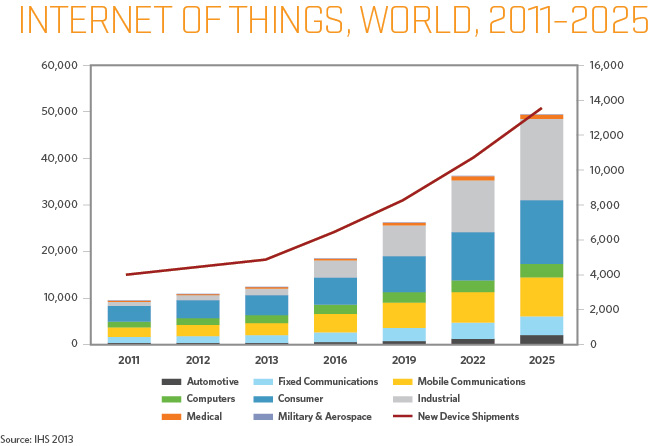
\includegraphics[scale=0.75]{graficoIot2011-2025}
\end{center}
\legend{Fonte: \citeauthor{ihs2013}, \citeyear{ihs2013} (Adaptado)}
\end{figure}

Tais dados se devem as consequências geradas pela emergência de tecnologias microeletrônicas, \textit{wireless} (\textit{Wi-fi}, \textit{Bluetooth} e \textit{ZigBee}), interfaces de comunicação móveis que se somaram as fixas já existentes e devido a formação de uma grande rede ubíqua capaz de conectar seres humanos com uma grande facilidade, possibilitando assim fornecer toda a base para a formação da IoT. \cite{santaella2013} 

\section{IoT}
\label{sec:iot}
No conceito de IoT um terceiro elemento foi inserido nas redes pervasivas que se possui hoje em dia, os objetos, sendo assim dentro da rede é possível se ter a comunicação entre humano-humano, humano-objeto e objeto-objeto, desta forma é possível ter humanos se comunicando normalmente como já acontecia anteriormente, humanos definindo comportamentos para os objetos e recebendo dados dos mesmos e objetos trocando informações entre si disponibilizando dados a humanos, dados estes, úteis para tomada de decisões ou até mesmo para facilitar atividades do dia a dia.\cite{santaella2013}

\begin{citacao}
Quando os objetos podem sentir o ambiente e se comunicar, eles se tornam ferramentas poderosas para entender coisas complexas e responder a elas com eficiência. Embora tais objetos inteligentes possam interagir com humanos, é mais provável que interajam ainda mais entre si automaticamente, sem intervenção humana atualizando-se com as tarefas do dia.\cite[p. 2]{presser2011}
\end{citacao}

Tais objetos podem ser considerados como tudo que está na rede e possui um endereçamento \textit{Internet Protocol} (IP), podendo interagir com outras interfaces endereçáveis dentro da mesma rede ou em outras através da internet, como mostra na figura \ref{fig:fluxogramaiot}.~\cite{ihs2013}

\begin{figure}[htb]
\caption{\label{fig:fluxogramaiot} Fluxograma da IoT}
\begin{center}
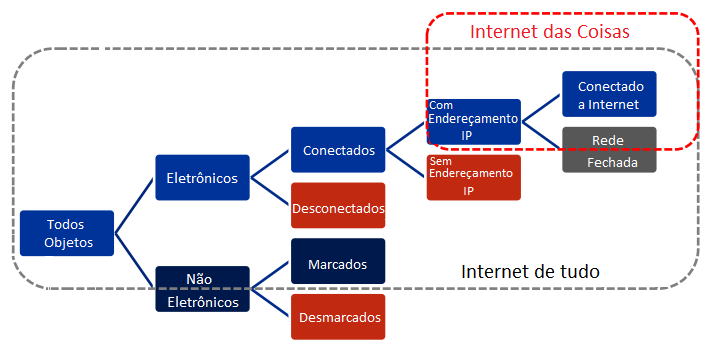
\includegraphics[scale=0.75]{fluxogramaiot}
\end{center}
\legend{Fonte: \citeauthor{ihs2013}, \citeyear{ihs2013} (Adaptado)} 
\end{figure}

Esses objetos podem ser um automóvel, uma geladeira, uma câmera, um sensor de temperatura, entre muitas outras interfaces, o que importa é que elas estão interligadas pela internet tomando ações de forma automática sem a intervenção humana. Pode-se citar o exemplo de um senhor que sofre de mal de Alzheimer e mora sozinho sendo que seus filhos não podem estar 24 horas por dia com ele, então os filhos decidem implantar sensores na casa do pai e pela vizinhança para que possam saber remotamente aonde ele está. Estes sensores estariam conectados a internet enviando dados para os filhos e emitindo alertas caso o pai saia de casa.\cite{presser2011}

Um outro exemplo de aplicação da IoT é apresentado na figura \ref{fig:exemploemergenciasiot}.

\begin{figure}[htb]
\caption{\label{fig:exemploemergenciasiot} Exemplo de aplicação da IoT}
\begin{center}
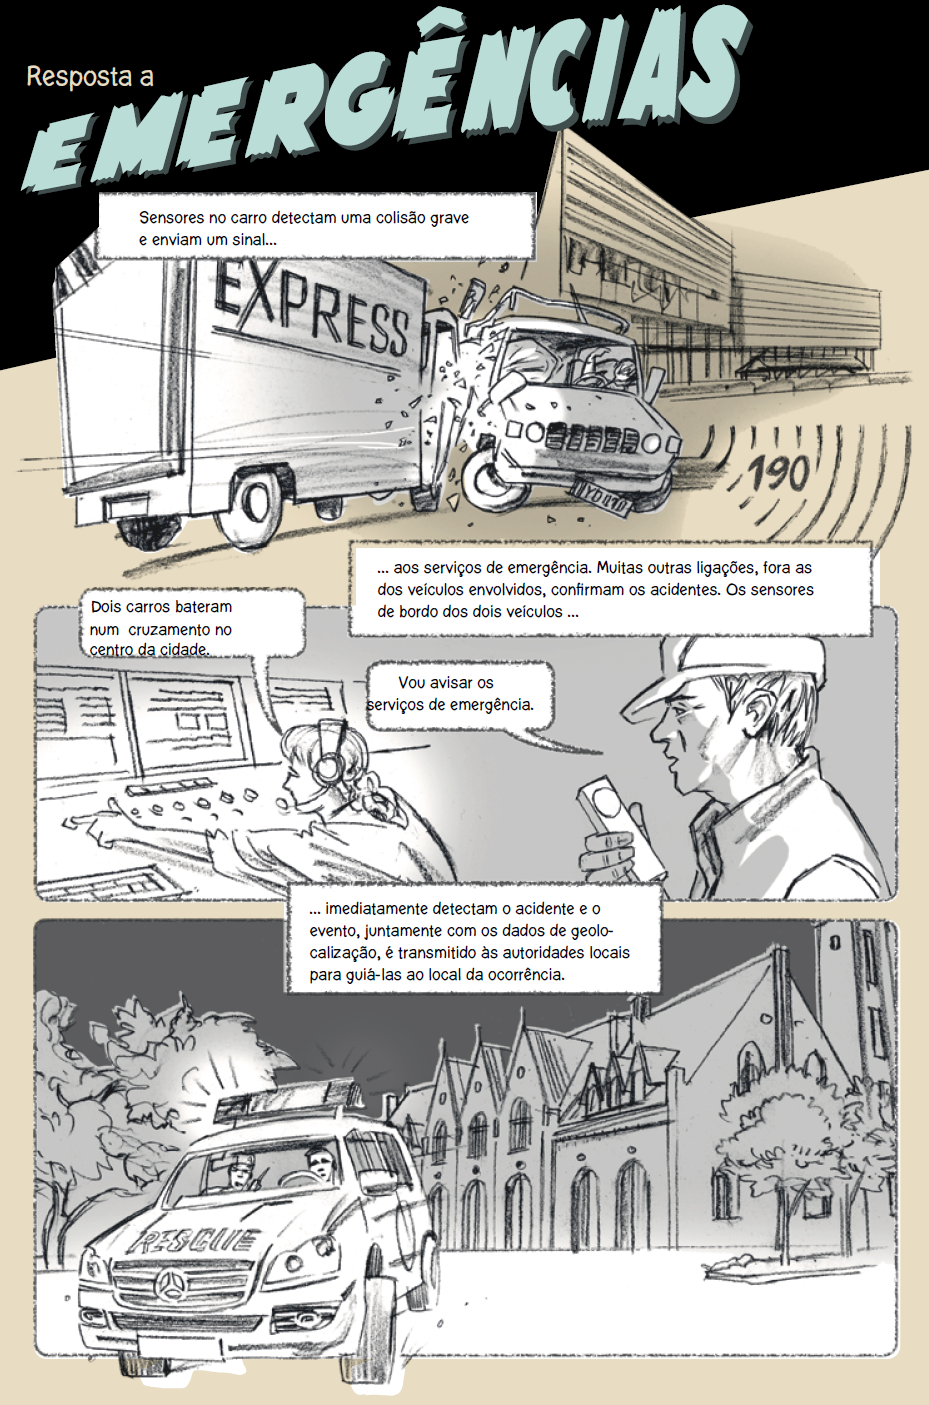
\includegraphics[scale=0.4]{exemploemergenciasiot}
\end{center}
\legend{Fonte: \citeauthor{presser2011}, \citeyear{presser2011} (Adaptado)} 
\end{figure}

Para que as aplicações de IoT tenha este tipo de comportamento é necessário que se tenha uma infraestrutura para dar suporte a esses objetos, ela pode ser estruturada de diferentes formas utilizando diversas tecnologias, mas de modo geral para o funcionamento de um sistema de IoT é necessário que se tenha os objetos conectados na internet ou a uma rede local, que envie e receba dados da infraestrutura (banco de dados ou armazenamento na nuvem) e os aplicativos que tem a função de gerenciar o sistema acessam e enviam os dados se comunicando diretamente com a infraestrutura, como é mostrado na figura~\ref{fig:estruturaiot}~\cite{ihs2013}

\begin{figure}[htb]
\caption{\label{fig:estruturaiot} Estrutura de um sistema de IoT}
\begin{center}
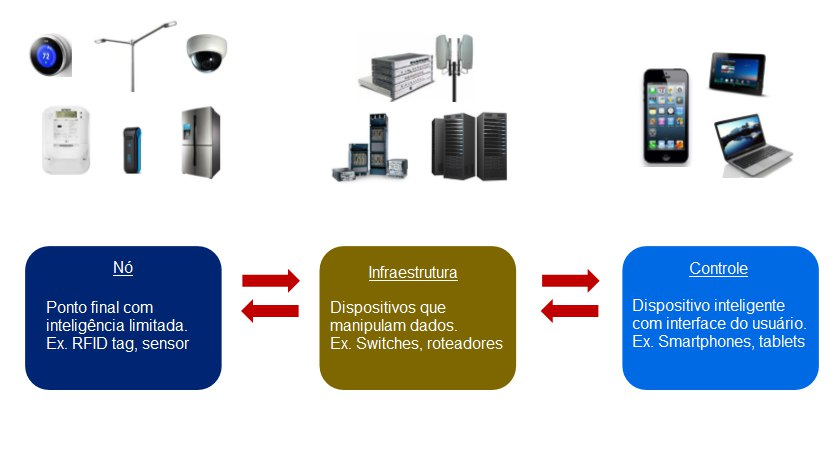
\includegraphics[scale=0.65]{estruturaiot}
\end{center}
\legend{Fonte: \citeauthor{ihs2013}, \citeyear{ihs2013} (Adaptado)} 
\end{figure}

\section{Cidades Inteligentes}
\label{sec:smartcities}
Com o grande crescimento da população como é possível ver na figura~\ref{fig:crescimentopopulacional}, as cidades também vem crescendo, mas de forma desordenada e desigual, causando problemas como o esgotamento de recursos, aumento da desigualdade social, aumento das áreas de favela, sem contar o caos com relação a locomoção dentro das cidades. Diante deste cenário criou-se o conceito de Cidades Inteligentes (\textit{Smart Cities}), que tem a finalidade de reinventar as cidades, ou seja reestruturá-las, a fim de que não haja desperdícios, tornando-a uma cidade sustentável e que a cidade seja organizada da melhor forma possível, trazendo uma melhor qualidade de vida aos cidadãos que nela vivem.\cite{leite2012cidades}

\begin{figure}[!h]
\caption{\label{fig:crescimentopopulacional} Impacto populacional}
\begin{center}
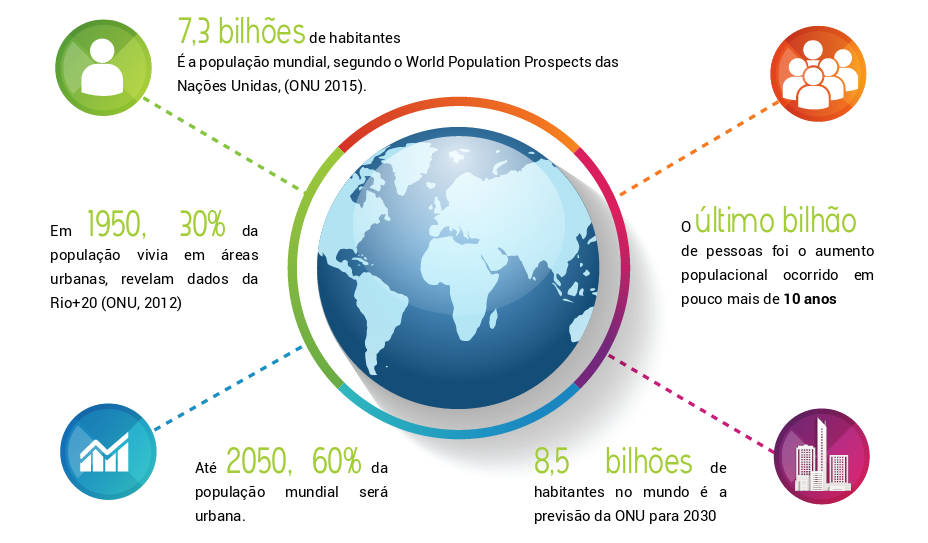
\includegraphics[scale=0.5]{crescimentopopulacional}
\end{center}
\legend{Fonte: \citeauthor{revistavia}, \citeyear{revistavia}} 
\end{figure}

Para tal reestruturação das cidades, transformando-as em Cidades Inteligentes, espera-se contar com o auxílio da área de Tecnologia da Informação e Comunicação (TIC), ou seja, boa parte das mudanças nas cidades se deverá pelo uso da tecnologia, mais especificamente pelas tecnologias de IoT. Elas poderão ajudar na redução de gases poluentes, redução na quantidade de lixo gerado pela população, redução do uso de recursos naturais, melhora da locomoção e segurança dentro das cidades, entre outras melhorias.\cite{leite2012cidades} 

\begin{citacao}
As maiores metrópoles do mundo têm adotado objetivos de tráfego e mobilidade para solucionar ou mitigar o problema de congestionamento com soluções de cidades inteligentes ativadas por Internet das Coisas (IoT), mas a mobilidade urbana não para em uma escolha contínua que consiste em se mover de A até B.~\cite[p. 1]{smartcities2017}.
\end{citacao}

\subsection{Mobilidade Urbana}
\label{subsec:mobilidadeurbana}
Dentro do conceito de Cidades Inteligentes, a mobilidade urbana se deve grande atenção, pois no século XXI ela tem se tornado um desafio a ser resolvido dentro das grandes cidades, pois o crescente número de veículos particulares causa um inchaço no trânsito, dificultando assim a locomoção, principalmente em grandes centros urbanos~\cite{gonccalomodelo}. Desta forma dentro de uma Cidade Inteligente a tecnologia pode ser aplicada para solucionar ou ao menos ser um paliativo aos problemas existentes, tecnologia esta que poderia atuar diretamente no trânsito, implantada através de \textit{smartphones} ou nos próprios carros, a fim de evitar acidentes, melhorar o fluxo, indicar rotas mais rápidas atuando diretamente na redução de gases poluentes e trazer maior facilidade aos motoristas.~\cite{gonccalomodelo}

\subsection{Saúde}
\label{subsec:saude}
Outro setor que se deve bastante atenção é o da saúde, pois é a necessidade básica da população, e infelizmente ela é muito precária nos dias de hoje, por diversos motivos principalmente os governamentais, mas através da tecnologia é possível que se mude este contexto. Com o uso de IoT é possível se criar aplicações na área da saúde que venha auxiliar no tratamento de doenças, cuidados com os pacientes, monitoramento e diagnósticos, transferência dos dados e colaboração, cadeiras de rodas inteligentes, Unidades de emergência conectadas, veículos de resposta, e hospitais, dentre tantas outras utilidades.~\cite{convergenciadigital}

Na área da saúde um grande desafio a se vencer é a de confiabilidade nos dados obtidos, pois um dado errado ou algo que se perca durante a transmissão pode representar a vida ou a morte de uma pessoa, visto que no futuro o uso de IoT na saúde será inevitável é necessário que se criem formas de manter esta tecnologia funcionando de forma segura e confiável.~\cite{convergenciadigital}

\section{V2V}
\label{sec:v2v}
Veiculo para Veiculo, ou V2V, habilita carros a se comunicarem entre eles em uma tentativa de avisar motoristas sobre potenciais acidentes ou colisões. A base da tecnologia é usar um onda de rádio de baixo alcance para permitir que os carros se comuniquem, podendo também que os carros enviem informações como localização, velocidade, direção, e também os estados dos freios, como mostra na figura~\ref{figsimulacao}.



\begin{figure}[!h]
\caption{\label{fig:simulacao} V2V simulação}
\begin{center}
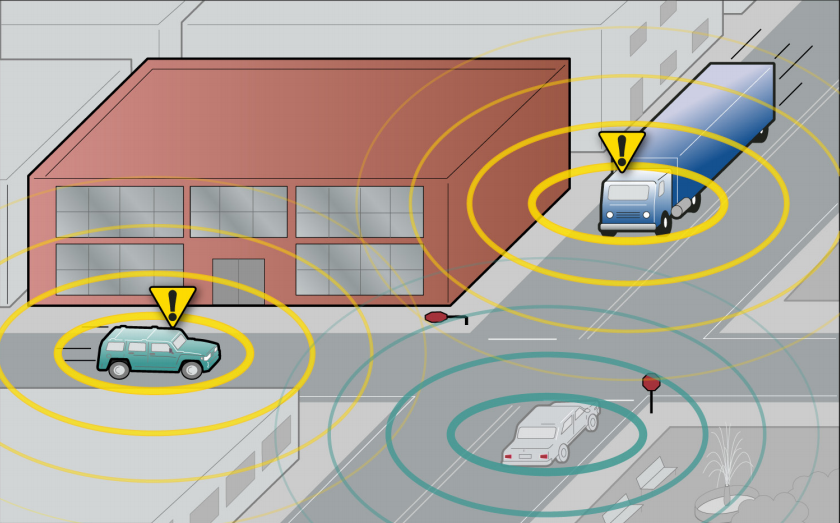
\includegraphics[scale=0.3]{v2v}
\end{center}
\legend{Fonte: \citeauthor{report2013}, \citeyear{report2013}} 
\end{figure}

\subsection{Regulamentação}
\label{subsec:regulamentacao}
Em dezembro de 2016 o Departamento de Transporte dos Estado Unidos (U.S. DOT) anunciou que esta trabalhando na regulamentação do uso da tecnologia em veículos de uso diário. O DOT diz que a tecnologia de rádio terá um alcance em média de 300 metros, e oferece um alcance maior que a abrangência de um radar ou câmera, em adição de não ser obstruídos por obstáculos ou outros veículos. O mesmo departamento acredita que a tecnologia poderá ser utilizada para avisar veículos sobre perigos eminentes particularmente quando se está em uma conversão ou realizando a troca de faixa. Adicionalmente, o departamento diz que os carros com sistemas automáticos de direção (ou até mesmo carros completamente autônomos) se beneficiaram das informações fornecidas pelo sistemas V2V.~\cite{usdot}

\section{V2I}
\label{sec:v2i}
Da mesma forma como acontece no caso do V2V, no paradigma de Veículo para Infraestrutura (V2I) os carros podem se comunicar, mas aqui a comunicação ocorre entre o carro e a infraestrutura, podendo receber instruções dela, assim como enviar instruções sobre as condições do veículo ou dados sobre o trânsito. A infraestrutura por sua vez, vem a ser as antenas que captam os dados do carro e os enviam para a nuvem, podendo usar estas informações transmitidas para se tomar decisões sobre o trânsito, analisar estatísticas, apontar trechos em que seja necessária a intervenção dos agentes de trânsito e trazer maior facilidade para o gerenciamento do mesmo.~\cite{howard2014}

Além da administração por parte dos agentes organizacionais, é possível que estes enviem mensagens para os carros a fim de alertar sobre algo á frente ou passar alguma informação relevante ao motorista, desta forma é possível notar as grandes vantagens trazidas por esse tipo de conexão que pode evitar acidentes e melhorar as condições do trânsito.~\cite{howard2014}

\subsection{Aplicação}
\label{subsec:aplicacao}
Como é apresentado em~\cite{tecmundo} hoje já é possível se ter exemplos da aplicação desta tecnologia, é o caso da empresa alemã Audi que está implantando nas próximas versões dos seus carros a tecnologia que ao parar em um semáforo inteligente, é exibido no painel do carro um temporizador indicando quanto tempo falta para abrir o semáforo, algo tido como não muito útil inicialmente, mas é só o começo do que há de vir, a ideia é avançar em busca de carros autônomos. 

O funcionamento deste sistema se dá pela comunicação do carro com as centrais de tráfego, instaladas nos semáforos, estas por sua vez se comunicam com os servidores, os quais enviam a informação que o veículo necessita, ao receber essas informações os veículos podem tomar ações, no caso de um carro autônomo (futuramente) ele poderia se preparar para uma parada no semáforo, trazendo maior economia de combustível.

Esta é uma tecnologia que tende a aumentar com o passar dos anos, pois no momento ainda é preciso que se reestruturem as cidades para que possa receber este tipo de tecnologia, como é o caso das centrais de tráfego, que atualmente não há este tipo de dispositivo instalado dentro das cidades, mas futuramente será algo necessário e que trará grandes benefícios a população podendo gerenciar o trânsito de forma inteligente evitando congestionamentos e gerenciando de forma mais eficiente o tempo dos semáforos.

\section{Funcionamento de Dispositivos de IoT}
\label{sec:dispositivosiot}
Quando se fala no uso de tecnologias IoT logo se pensa em sensores conectados na rede captando dados, sendo assim é preciso se detalhar o que são estes dispositivos e como funcionam.

\subsection{Sensores}
\label{subsec:sensores}
Sensor é o termo para designar um dispositivo sensível a algum tipo de energia do ambiente, podendo ela ser luminosa, térmica, cinética, relacionado a uma grandeza física como temperatura, pressão velocidade, corrente, aceleração, etc. Normalmente o sinal de saída de um sensor deve ser manipulado antes de sua utilização, geralmente através do uso de um amplificador, pois as tensões de saída após o dispositivo ser sensibilizado costumam ser baixas.~\cite{wendling2010}

\subsection{Transdutores}
\label{subsec:transdutores}
É o termo designado para se referenciar o dispositivo que transforma um tipo de energia em outra, trabalham geralmente junto com os sensores transformando o impulso elétrico vindo dos sensores em valores digitais úteis dentro de um sistema de IoT. Um exemplo de transdutor é o alto-falante que converte o impulso elétrico em movimento mecânico necessário para reproduzir o som.~\cite{wendling2010}


%\autoref{chap:cap1}
% ---
%\section{Aliquam vestibulum fringilla lorem}
%\lipsum[2]
%\subsection{Subsessão cap 1}
%\lipsum[2]
%\chapter{Capitulo Segundo}
%\lipsum[2]
